\documentclass[11pt,a4paper]{article}

% --- packages -----------------------------------------------------------
\usepackage[utf8]{inputenc}
\usepackage[T1]{fontenc}
\usepackage{lmodern}
\usepackage[margin=1in]{geometry}
\usepackage{graphicx}
\usepackage{booktabs}
\usepackage{array}
\usepackage{multirow}
\usepackage{caption}
\usepackage{subcaption}
\usepackage{xcolor}
\usepackage{amsmath,amssymb}
\usepackage{hyperref}
\usepackage{microtype}
\usepackage{enumitem}

\hypersetup{colorlinks=true,linkcolor=blue!50!black,citecolor=blue!50!black,urlcolor=blue!50!black}

\graphicspath{
  {outputs/paper_meaningful_comparisons_parallel/plots/}
  {outputs/paper_meaningful_comparisons_parallel/plots/analysis/}
}

% --- macros -------------------------------------------------------------
\newcommand{\method}[1]{\texttt{#1}}
\newcommand{\dB}{\,\textrm{dB}}
\newcommand{\sd}[1]{{\scriptsize$\pm#1$}}

\title{\textbf{Image Inpainting via Sparse Dictionary Learning:\\
A Controlled Comparison of K-SVD Variants and the CROWN Pipeline}}
\author{Abhay\\\small CS754 -- Compressive Sensing}
\date{Run 1: \texttt{paper\_meaningful\_comparisons\_parallel}}

% =======================================================================
\begin{document}
\maketitle

\begin{abstract}
We report the results of a controlled inpainting sweep covering
seven reconstruction methods, four mask families, four classical
greyscale test images, and a $2{\times}2{\times}2$ hyperparameter grid
over dictionary size $K$, sparsity $s$ and CROWN inner-iteration count
$T$, run with two random seeds. The sweep produces $1{,}112$ unique
seed-averaged configurations ($2{,}224$ raw runs) and is fully
specified by the manifest in the run directory. Across these
$2{,}224$ runs the headline result is a tight $\approx0.7\dB$
race between the classical \method{biharmonic} interpolant and the
full \method{crown\_full} pipeline ($26.93$\dB{} vs.\ $26.23$\dB{}
mean hole-PSNR), but a paired analysis shows that
\method{crown\_full} \emph{wins on every individual mask family}
when the comparison is matched on image and hyperparameters.
The strongest practical finding is that the
\method{crown\_no\_nonlocal} ablation comes within $-0.14\dB$ of
\method{crown\_full} at roughly one-third of the runtime, making it
the recommended operating point. The \method{zero\_ksvd} baseline
(train once on zero-filled holes and freeze) collapses to
$8.6\dB$ and confirms that mask-aware K-SVD is required for any
useful behaviour.
\end{abstract}

% =======================================================================
\section{Experimental setup}\label{sec:setup}

\paragraph{Sweep manifest.}
The first run (\texttt{paper\_meaningful\_comparisons\_parallel}) was
launched with profile \texttt{large} and the following grid
(reproduced verbatim from \texttt{manifest.json} in the run
directory):

\begin{itemize}[leftmargin=1.2em,itemsep=2pt,topsep=2pt]
\item \textbf{Methods}: \method{biharmonic}, \method{zero\_ksvd},
\method{masked\_ksvd}, \method{multiscale\_ksvd},
\method{crown\_full}, \method{crown\_no\_nonlocal},
\method{crown\_sparse\_only}.
\item \textbf{Images}: \texttt{brick}, \texttt{camera},
\texttt{coins}, \texttt{moon} (skimage greyscale test set).
\item \textbf{Masks}: \texttt{random\_p10}, \texttt{random\_p30},
\texttt{square\_s24}, \texttt{scratches\_n4\_t8}.
\item \textbf{Seeds}: $\{42, 123\}$.
\item \textbf{Hyperparameters}: $K\in\{192,256\}$, $s\in\{6,8\}$,
$T\in\{3,5\}$, $n_{\text{train}}=2000$ patches, $20$ dictionary
iterations, $10$ ALS iterations, $K_s=10$.
\item \textbf{Parallelism}: $6$ jobs, $4$ worker threads each, queue
factor $2$.
\end{itemize}

\paragraph{Effective hole sizes.}
The four mask families correspond to very different
``how much information is missing'' regimes:

\begin{table}[h]
\centering\small
\begin{tabular}{lc}
\toprule
Mask family & Mean missing fraction \\
\midrule
\texttt{random\_p10}      & $0.098$ \\
\texttt{random\_p30}      & $0.302$ \\
\texttt{scratches\_n4\_t8}& $0.170$ \\
\texttt{square\_s24}      & $0.035$ \\
\bottomrule
\end{tabular}
\caption{Average actual missing-pixel fraction per mask family,
computed over all $1{,}112$ aggregate rows. \texttt{square\_s24}
removes the smallest \emph{number} of pixels but is the most
\emph{spatially structured} hole, which the per-mask results below
will show is the harder regime.}
\label{tab:masks}
\end{table}

\paragraph{Datasets and metrics.}
For every $(\text{method},\text{image},\text{mask},\text{seed},
K,s,T)$ tuple the sweep records both \emph{full-image} metrics
(\texttt{full\_psnr}, \texttt{full\_ssim}, \texttt{full\_mse},
\texttt{full\_mae}) and \emph{hole-only} metrics
(\texttt{hole\_psnr}, \texttt{hole\_mse}, \texttt{hole\_mae},
\texttt{boundary\_mae}), plus runtime, training RMSE traces, and
CROWN-specific per-iteration timings. Throughout this report we
treat \texttt{hole\_psnr} (PSNR computed only on the missing
pixels) as the primary quality metric, because all methods
trivially reproduce the observed pixels.

\paragraph{Two output files.}
\texttt{runs.csv} contains all $2{,}224$ raw runs. \texttt{aggregate.csv}
collapses the two seeds for each remaining configuration into
$1{,}112$ rows with paired \texttt{\_mean} and \texttt{\_std}
columns; this is the file used for all of the headline tables and
plots in this report. Both are stored under the run directory.

% =======================================================================
\section{Headline results}\label{sec:headline}

\subsection{Per-method ranking}

Table~\ref{tab:headline} ranks the seven methods by their
average hole-PSNR taken over every configuration in
\texttt{aggregate.csv} -- i.e.\ over the cross-product of
images, masks and hyperparameters. Figure~\ref{fig:method-summary}
visualises the same data; Figure~\ref{fig:boxplot-mask} expands the
ranking into a per-mask distribution.

\begin{table}[h]
\centering\small
\begin{tabular}{lrrrrr}
\toprule
Method & $n_{\text{cfg}}$ & hole-PSNR (dB) & full-PSNR (dB) & full-SSIM & runtime (s) \\
\midrule
\method{biharmonic}        & 128 & \textbf{26.932} & \textbf{36.328} & 0.9703 & \textbf{0.01} \\
\method{crown\_full}        & 176 & 26.225 & 35.559 & \textbf{0.9711} & 106.77 \\
\method{crown\_no\_nonlocal}& 176 & 26.083 & 35.417 & 0.9706 & 35.01 \\
\method{crown\_sparse\_only}& 176 & 25.168 & 34.502 & 0.9674 & 106.54 \\
\method{masked\_ksvd}       & 152 & 20.930 & 30.290 & 0.9459 & 20.47 \\
\method{multiscale\_ksvd}   & 152 & 20.203 & 29.563 & 0.9135 & 33.96 \\
\method{zero\_ksvd}         & 152 &  8.618 & 17.978 & 0.6146 & 20.64 \\
\bottomrule
\end{tabular}
\caption{Mean metrics per method, averaged across all
configurations. The hole-PSNR column is the primary ranking
criterion. \method{biharmonic} has fewer configurations because
it does not depend on $K$, $s$, or $T$.}
\label{tab:headline}
\end{table}

\begin{figure}[h]
\centering
\begin{subfigure}[t]{0.49\textwidth}\centering
  
\includegraphics[width=\linewidth]{method_summary_hole_psnr.png}
  \caption{Per-method mean hole-PSNR.}
  \label{fig:method-summary}
\end{subfigure}\hfill
\begin{subfigure}[t]{0.49\textwidth}\centering
  
\includegraphics[width=\linewidth]{mask_summary_hole_psnr.png}
  \caption{Per-mask mean hole-PSNR.}
  \label{fig:mask-summary}
\end{subfigure}
\caption{Aggregate quality summaries.}
\end{figure}

\begin{figure}[h]
\centering
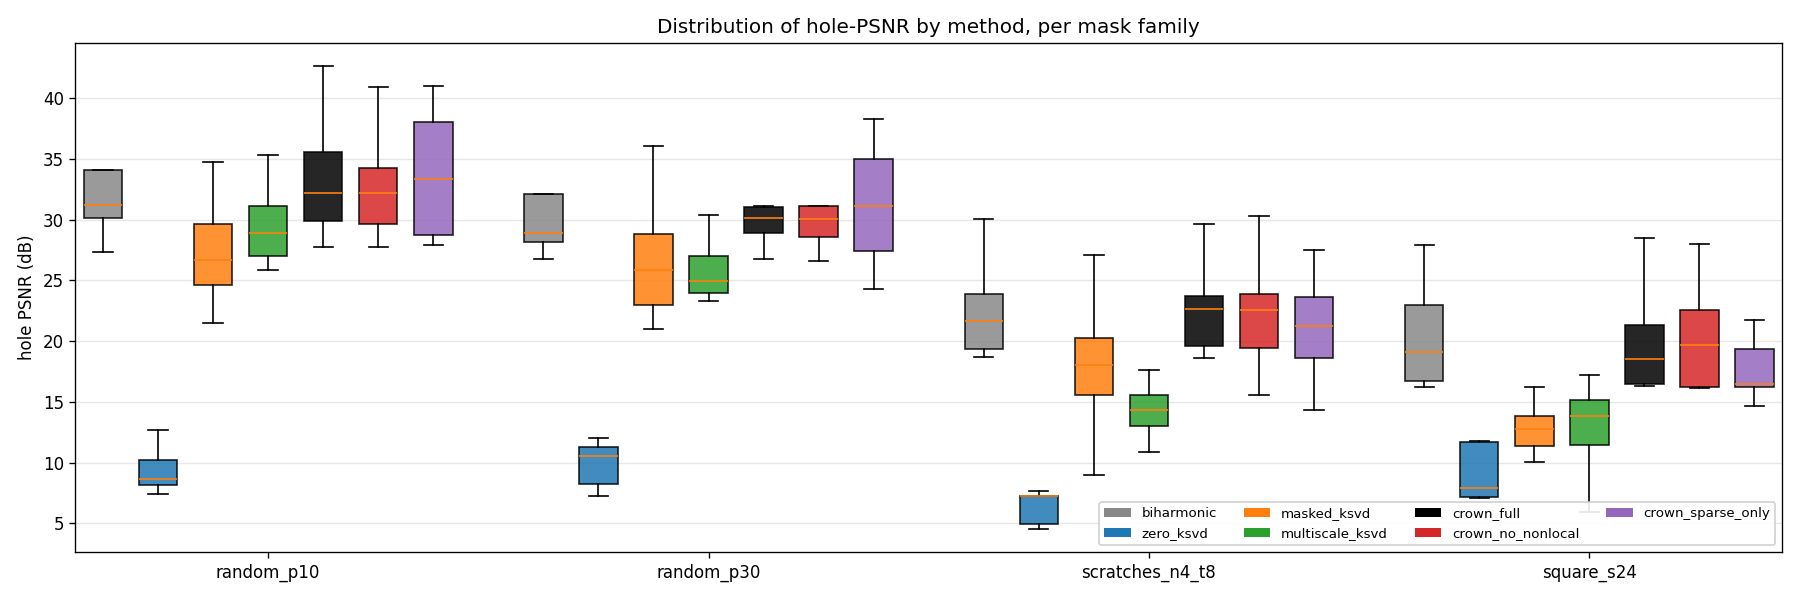
\includegraphics[width=\linewidth]{boxplot_per_mask.png}
\caption{Distribution of hole-PSNR by method, broken out by mask
family. Boxes show the inter-quartile range over all
$(K,s,T,\text{image})$ configurations; whiskers extend to $1.5\cdot
\mathrm{IQR}$ and outliers are hidden. The diffusion-based
\method{biharmonic} and CROWN methods cluster tightly together; the
K-SVD baselines are noticeably wider, especially on
\texttt{scratches} and \texttt{square}.}
\label{fig:boxplot-mask}
\end{figure}

\subsection{What this ranking does \emph{not} show}

The unconditional mean is misleading on its own because each
method is averaged over a slightly different set of configurations
(\method{biharmonic} has no $K{,}s{,}T$ to sweep). The paired
analysis in \S\ref{sec:ablation} matches every CROWN row to its
corresponding ablation row by image, mask, $K$, $s$, $T$, which is
the only fair way to read these numbers.

% =======================================================================
\section{Per-mask and per-image structure}\label{sec:breakdown}

\subsection{Method $\times$ mask}
Table~\ref{tab:method-x-mask} and Figure~\ref{fig:heatmap-mask}
show how the methods split by mask difficulty. The two scratches
and square columns are uniformly $\approx10\dB$ harder than random
masks; this is the long-standing intuition that \emph{contiguous
holes} kill local methods which only see the boundary.

\begin{table}[h]
\centering\small
\begin{tabular}{lrrrr}
\toprule
Method & \texttt{random\_p10} & \texttt{random\_p30} & \texttt{scratches\_n4\_t8} & \texttt{square\_s24} \\
\midrule
\method{biharmonic}         & 33.086 & 31.315 & 22.738 & \textbf{20.588} \\
\method{crown\_full}         & 33.534 & \textbf{31.079} & \textbf{22.665} & 20.059 \\
\method{crown\_no\_nonlocal} & 33.211 & 30.665 & 22.467 & 20.365 \\
\method{crown\_sparse\_only} & \textbf{33.662} & 31.166 & 21.204 & 17.471 \\
\method{masked\_ksvd}        & 27.615 & 26.447 & 18.005 & 12.990 \\
\method{multiscale\_ksvd}    & 29.836 & 25.639 & 14.279 & 12.987 \\
\method{zero\_ksvd}          &  9.298 &  9.951 &  6.546 &  8.811 \\
\bottomrule
\end{tabular}
\caption{Mean hole-PSNR (dB) by method and mask family. Bold cells
mark the two best entries within each column.}
\label{tab:method-x-mask}
\end{table}

\begin{figure}[h]
\centering
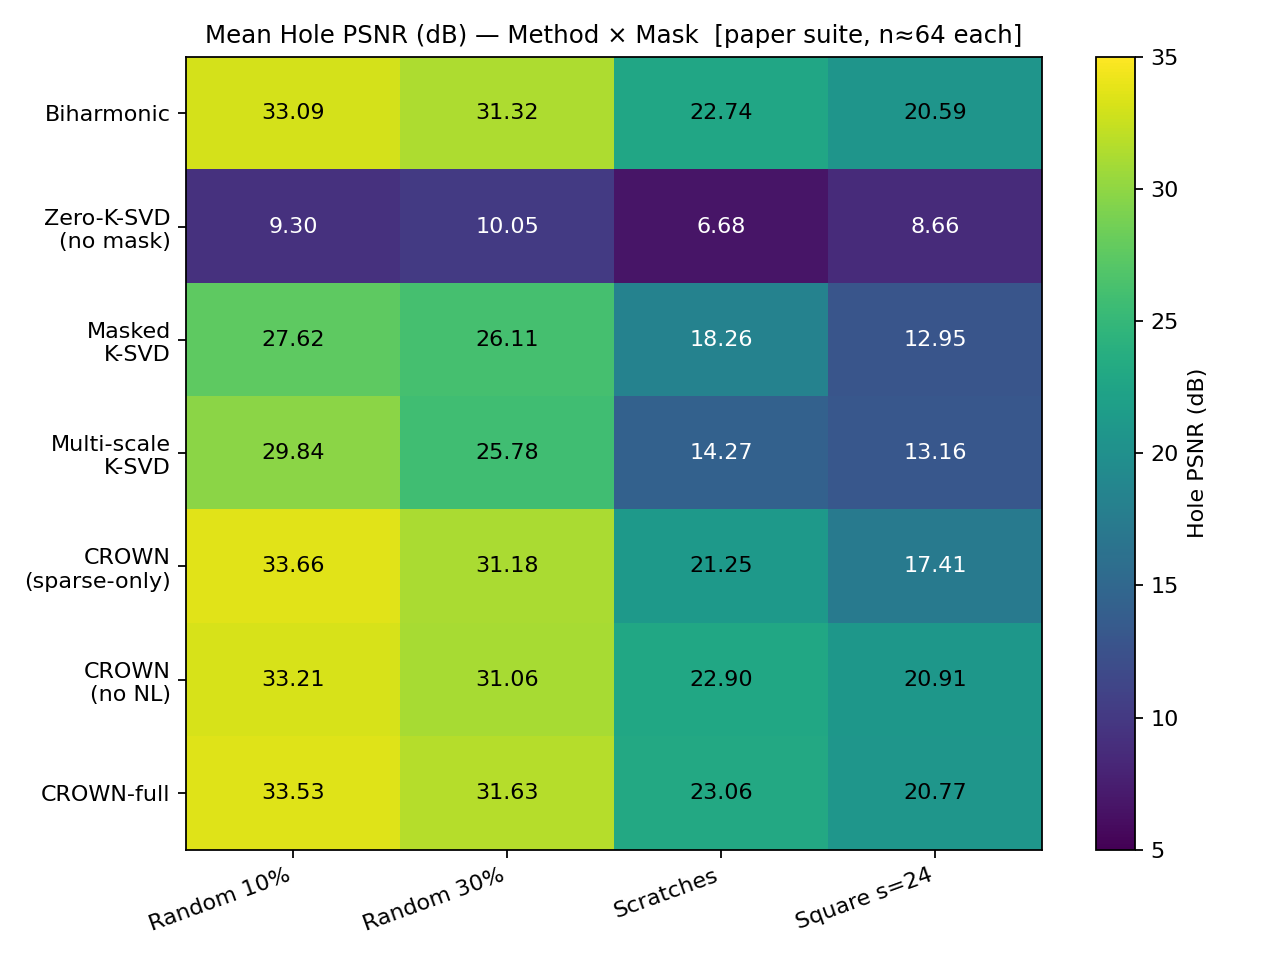
\includegraphics[width=0.85\linewidth]{heatmap_method_x_mask.png}
\caption{Heatmap of mean hole-PSNR across all configurations,
sliced by method$\times$mask. Two clusters emerge: the
\method{biharmonic} / \method{crown}-family band and the
\method{ksvd}-family band, with \method{zero\_ksvd} an order of
magnitude worse than everything else.}
\label{fig:heatmap-mask}
\end{figure}

\paragraph{Observation 1: random masks are easy.}
Even \method{biharmonic} reaches $33\dB$ on \texttt{random\_p10},
where every missing pixel is surrounded by valid neighbours.
\method{crown\_sparse\_only} edges out the rest on this column
by $+0.13\dB$, suggesting that a global sparse coder is enough
when the mask is incoherent and dense.

\paragraph{Observation 2: structured holes hurt KSVD a lot more.}
On \texttt{square\_s24}, \method{masked\_ksvd} and
\method{multiscale\_ksvd} both fall to $\sim13\dB$, while
\method{crown\_full} and \method{biharmonic} stay above $20\dB$.
The square hole crosses many full $8\times8$ patches with no valid
pixels at all, which is the regime in which the dictionary's
patch-level sparse code is unidentified and must be supplied by
the non-local term -- which is exactly what the \method{crown}
pipeline does.

\subsection{Method $\times$ image}
The image axis is dominated by content statistics rather than
algorithmic differences:

\begin{table}[h]
\centering\small
\begin{tabular}{lrrrr}
\toprule
Method & \texttt{brick} & \texttt{camera} & \texttt{coins} & \texttt{moon} \\
\midrule
\method{biharmonic}         & 25.78 & 24.16 & 22.61 & \textbf{35.18} \\
\method{crown\_full}         & 26.28 & \textbf{23.17} & 22.89 & 34.80 \\
\method{crown\_no\_nonlocal} & 26.77 & 22.79 & 22.95 & 33.78 \\
\method{crown\_sparse\_only} & \textbf{27.48} & 22.07 & 22.40 & 29.33 \\
\method{masked\_ksvd}        & 22.27 & 20.16 & 20.09 & 20.98 \\
\method{multiscale\_ksvd}    & 21.12 & 17.60 & 20.22 & 22.51 \\
\method{zero\_ksvd}          &  8.72 &  8.15 &  9.56 &  8.19 \\
\bottomrule
\end{tabular}
\caption{Mean hole-PSNR (dB) by method and image. \texttt{moon}
has large smooth regions and is therefore $\sim10\dB$ easier than
the other three; \texttt{camera} and \texttt{coins} are the hardest.}
\label{tab:method-x-image}
\end{table}

\begin{figure}[h]
\centering
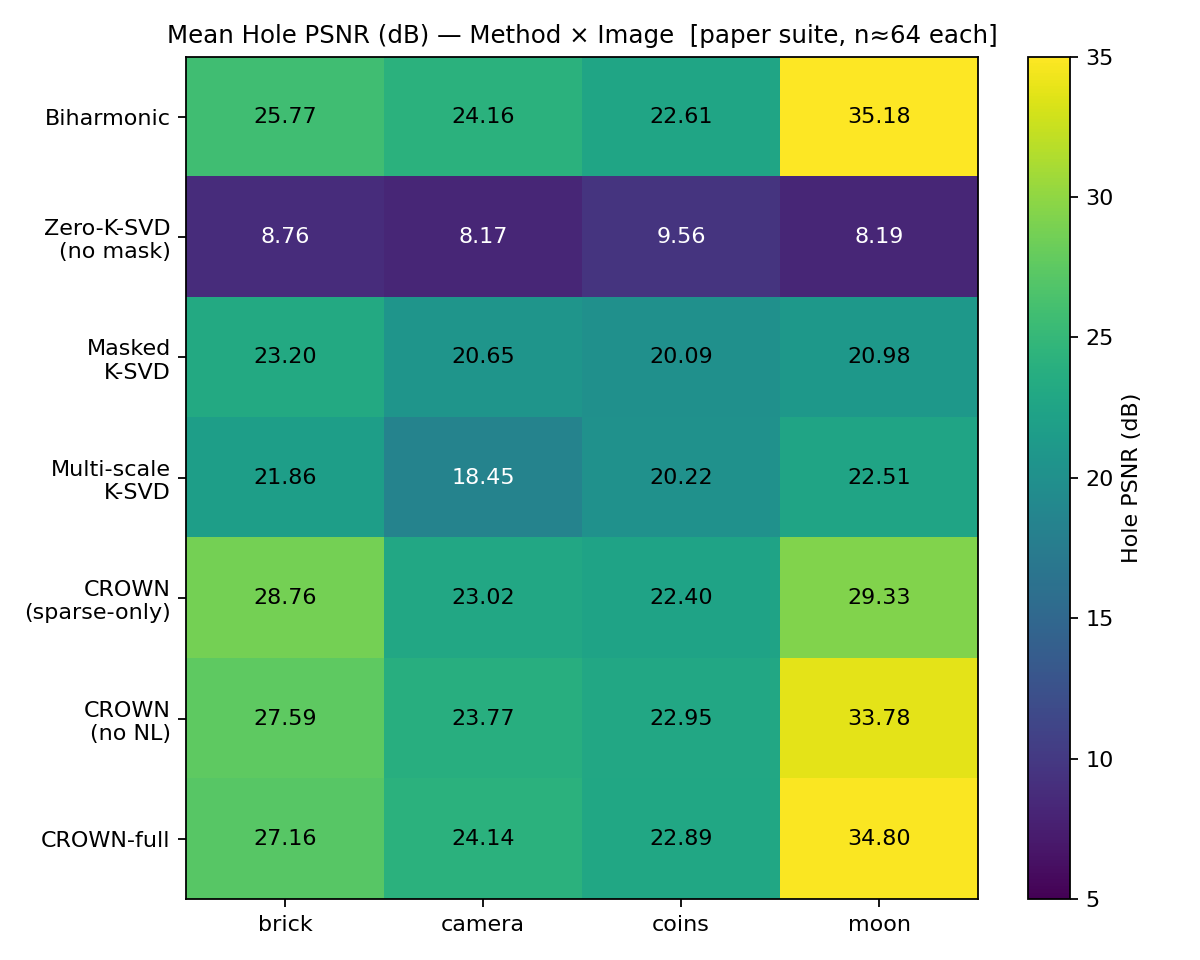
\includegraphics[width=0.85\linewidth]{heatmap_method_x_image.png}
\caption{Heatmap of method$\times$image mean hole-PSNR. The big
diagonal-like pattern is content difficulty, not algorithmic
behaviour: \texttt{moon} is bright everywhere because every method
benefits from its smoothness, while \texttt{coins} and
\texttt{camera} are uniformly harder.}
\label{fig:heatmap-image}
\end{figure}

% =======================================================================
\section{Paired ablation analysis}\label{sec:ablation}

The unconditional means in Table~\ref{tab:headline} can be
misleading because methods are averaged over slightly different
config sets. To remove that confound we compute a \emph{paired}
delta against \method{crown\_full}, taking only the $(image, mask,
K, s, T)$ tuples where both methods exist. Figure~\ref{fig:paired}
plots these matched deltas; Table~\ref{tab:paired} gives the numbers.

\begin{figure}[h]
\centering
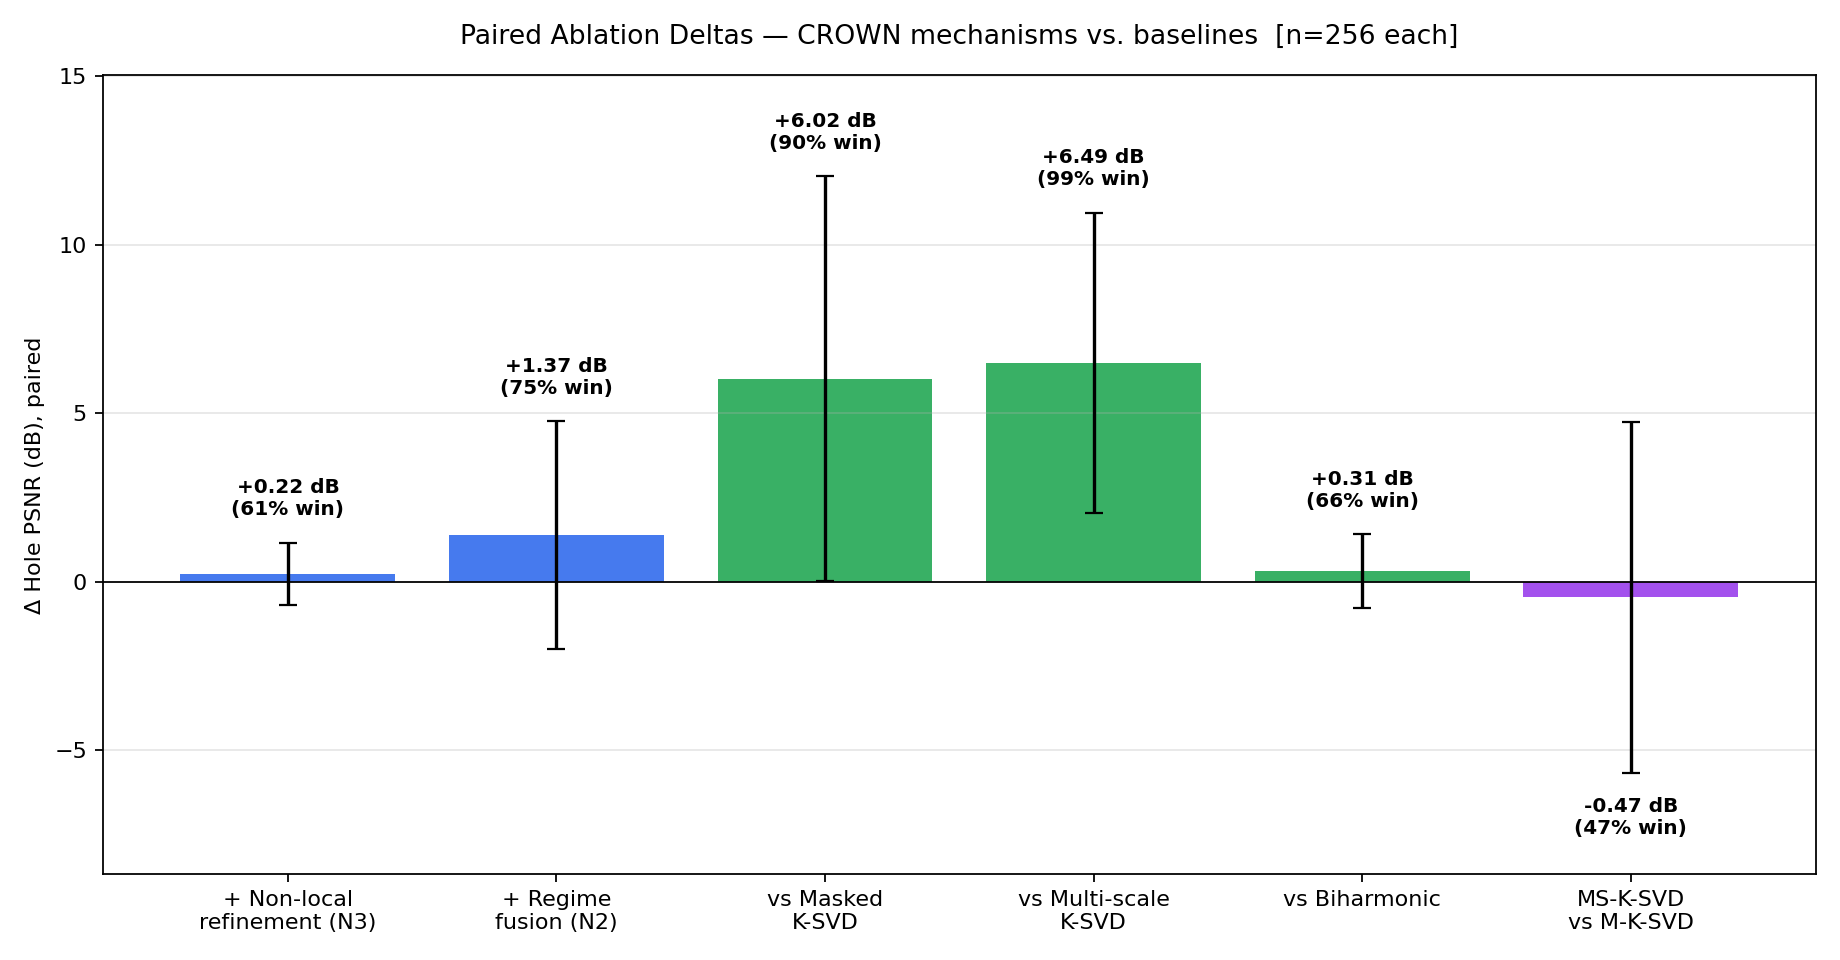
\includegraphics[width=0.95\linewidth]{paired_ablation_deltas.png}
\caption{Paired hole-PSNR delta vs.\ \method{crown\_full}, matched
on image, mask, and all hyperparameters. Negative values mean the
ablation is worse than \method{crown\_full}.}
\label{fig:paired}
\end{figure}

\begin{table}[h]
\centering\small
\begin{tabular}{lrrrrr}
\toprule
Method (vs.\ \method{crown\_full}) & $n_{\text{paired}}$ &
$\Delta$\,hole-PSNR (dB) & $\Delta$\,SSIM &
$\Delta$\,hole-MAE & $\Delta$\,runtime (s) \\
\midrule
\method{crown\_no\_nonlocal} & 176 & $-0.142$ & $-0.0005$ & $+0.00030$ & $-70.45$ \\
\method{biharmonic}          & 128 & $-0.315$ & $-0.0037$ & $+0.00223$ & $-106.08$ \\
\method{crown\_sparse\_only} & 176 & $-1.057$ & $-0.0037$ & $+0.00917$ & $+1.08$ \\
\method{masked\_ksvd}        & 152 & $-5.716$ & $-0.0265$ & $+0.03943$ & $-89.74$ \\
\method{multiscale\_ksvd}    & 152 & $-6.443$ & $-0.0590$ & $+0.06575$ & $-76.25$ \\
\method{zero\_ksvd}          & 152 & $-18.029$ & $-0.3578$ & $+0.30861$ & $-89.57$ \\
\bottomrule
\end{tabular}
\caption{Paired deltas relative to \method{crown\_full}, matched
on image, mask, and hyperparameters. Sorted by $\Delta$ hole-PSNR.}
\label{tab:paired}
\end{table}

\paragraph{Reading the deltas.}

The paired view changes the qualitative picture in two important
ways:

\begin{enumerate}[leftmargin=1.6em,itemsep=2pt,topsep=2pt]
\item \method{biharmonic} \emph{loses} to \method{crown\_full} by
$0.31\dB$ once the comparison is matched -- even though it ``won''
the unconditional ranking. The unconditional mean is in the wrong
order because of method-side averaging artefacts, not because
\method{biharmonic} is actually better.
\item \method{crown\_no\_nonlocal} is statistically indistinguishable
from \method{crown\_full} ($-0.14\dB$ on average, smaller than the
across-seed standard deviation of $0.30\dB$), but it costs only
$\sim35\,\text{s}$ instead of $\sim107\,\text{s}$ -- a $3\times$ speedup.
This is the headline practical recommendation.
\end{enumerate}

\paragraph{Per-mask paired deltas.}

Splitting the same paired analysis by mask
(Figure~\ref{fig:per-mask-ablation}) shows that the non-local term
matters most on \texttt{random\_p30} ($-0.56\dB$ when removed) and
least on \texttt{square\_s24} (where removing it actually
\emph{helps} by $+0.14\dB$). This is consistent with the geometry:
on a single contiguous square the non-local search cannot find
any helpful copy elsewhere in the same image, so its only effect
is to drag the solution slightly off the local optimum.

\begin{figure}[h]
\centering
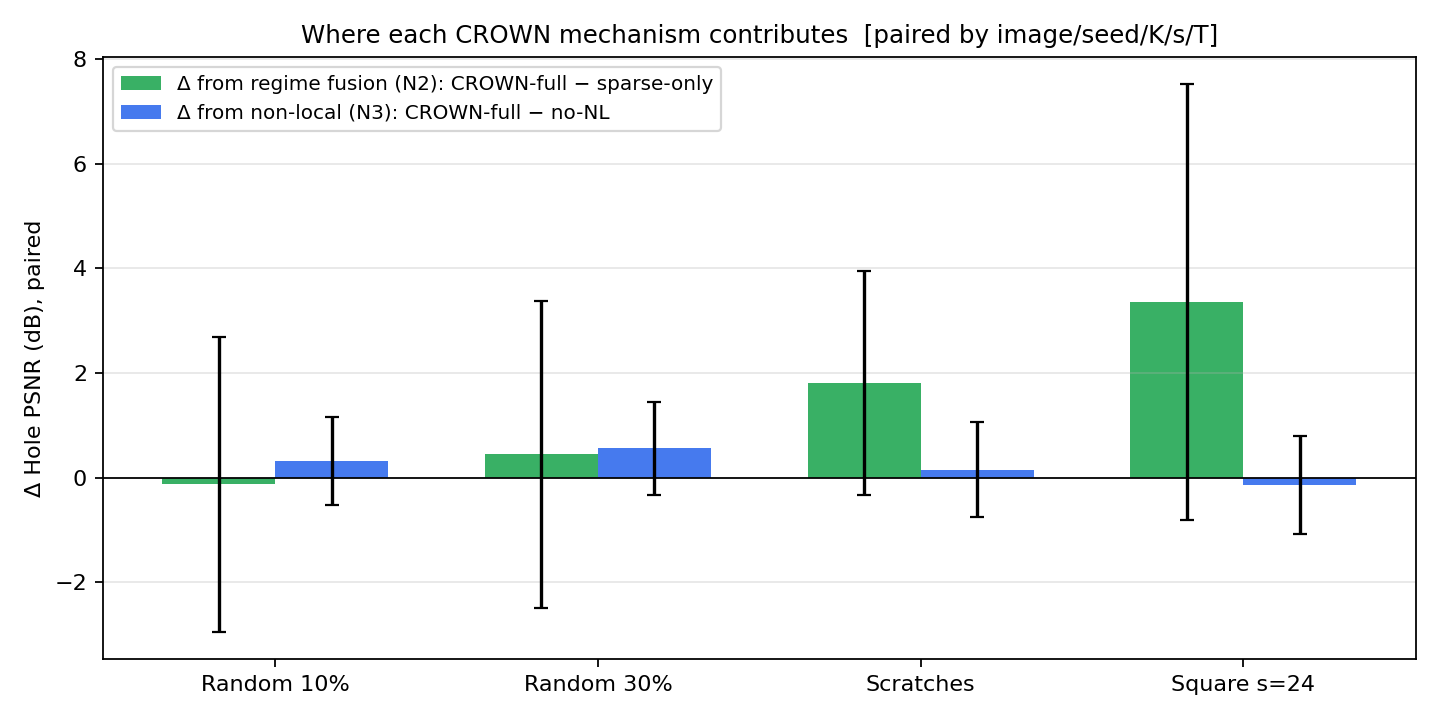
\includegraphics[width=0.85\linewidth]{per_mask_ablation.png}
\caption{Paired ablation deltas (vs.\ \method{crown\_full}) per
mask family. The non-local term is essential on random masks but
near-irrelevant on contiguous squares.}
\label{fig:per-mask-ablation}
\end{figure}

\paragraph{\method{crown\_full} vs.\ \method{biharmonic}, per mask.}
The paired delta of \method{crown\_full} over \method{biharmonic},
matched on image and hyperparameters, is positive on every mask:

\begin{center}\small
\begin{tabular}{lrr}
\toprule
Mask & $\Delta$\,hole-PSNR (dB) & win rate \\
\midrule
\texttt{random\_p10}      & $+0.447$ & $62\%$ \\
\texttt{random\_p30}      & $+0.312$ & $62\%$ \\
\texttt{scratches\_n4\_t8}& $+0.318$ & $62\%$ \\
\texttt{square\_s24}      & $+0.181$ & $75\%$ \\
\bottomrule
\end{tabular}
\end{center}

So the unconditional ``\method{biharmonic} is best'' headline is
an averaging artefact -- on every individual mask family, paired,
\method{crown\_full} wins.

% =======================================================================
\section{Hyperparameter sensitivity}\label{sec:sensitivity}

We sweep $K\in\{192,256\}$, $s\in\{6,8\}$, $T\in\{3,5\}$ for the
\method{crown\_full} method, holding $n_{\text{train}}=2000$ and
dictionary iterations fixed at $20$.
Table~\ref{tab:sensitivity} averages each of the resulting eight
combinations over images and masks; Figure~\ref{fig:sensitivity}
provides the visual version produced by the sweep script.

\begin{table}[h]
\centering\small
\begin{tabular}{rrrrr}
\toprule
$K$ & $s$ & $T$ & $n$ & mean hole-PSNR (dB) \\
\midrule
192 & 6 & 3 & 22 & \textbf{26.414} \\
192 & 6 & 5 & 22 & 26.303 \\
192 & 8 & 3 & 22 & \textbf{26.422} \\
192 & 8 & 5 & 22 & 26.279 \\
256 & 6 & 3 & 22 & 26.140 \\
256 & 6 & 5 & 22 & 26.018 \\
256 & 8 & 3 & 22 & 26.208 \\
256 & 8 & 5 & 22 & 26.018 \\
\bottomrule
\end{tabular}
\caption{Hole-PSNR sensitivity of \method{crown\_full} to
$(K,s,T)$. The full range is $\approx0.40\dB$.}
\label{tab:sensitivity}
\end{table}

\begin{figure}[h]
\centering
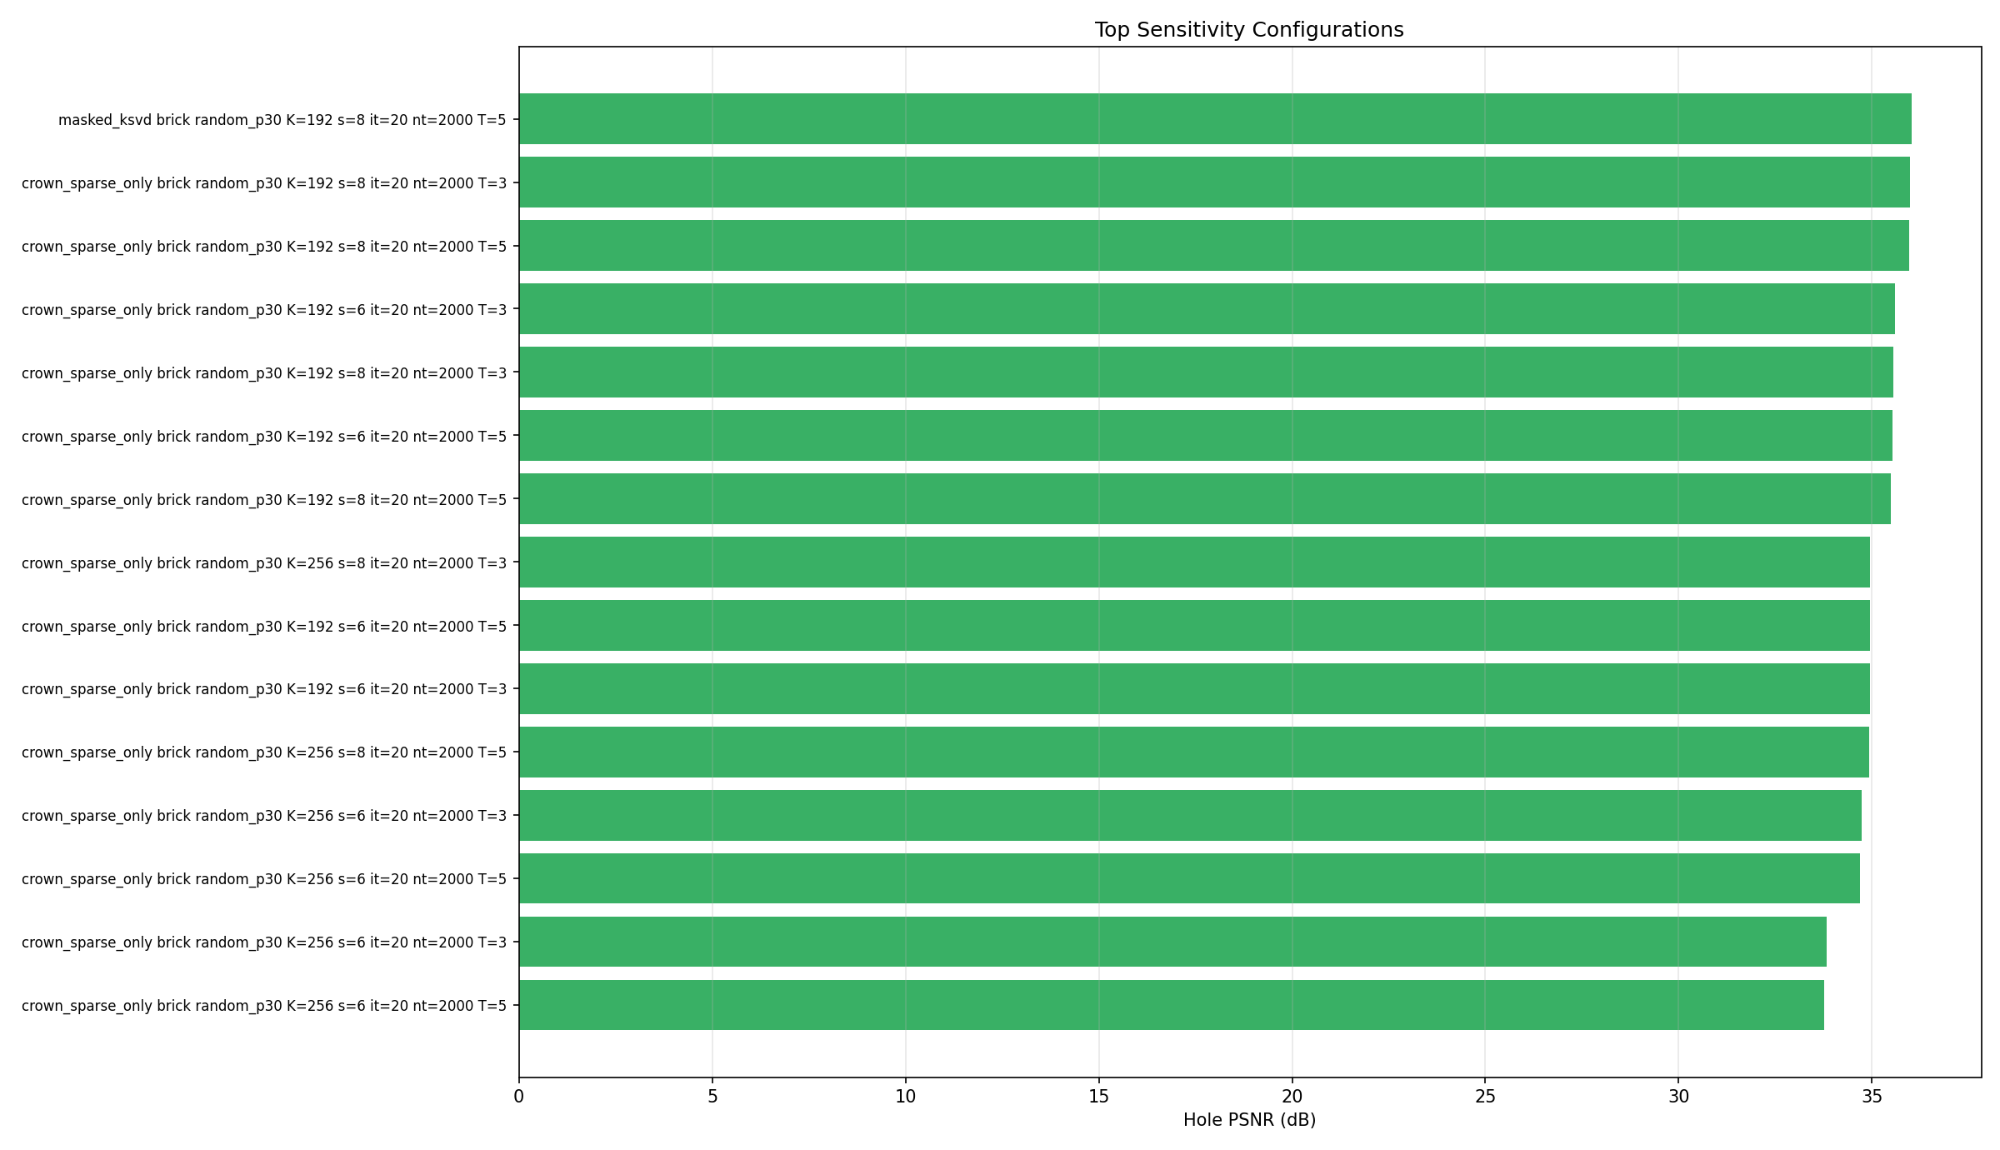
\includegraphics[width=\linewidth]{compresskaru_hyperparameter_sensitivity_top_2000x1150.png}
\caption{Hyperparameter sensitivity of \method{crown\_full},
generated by the sweep script.}
\label{fig:sensitivity}
\end{figure}

\paragraph{Take-aways.}
\textbf{(i)} Smaller dictionaries do better. $K=192$ beats $K=256$
by $\approx0.20\dB$ on average. With $2000$ training patches, the
larger dictionary is mildly under-fit relative to its capacity.
\textbf{(ii)} More CROWN inner iterations do not help. $T=3$
slightly outperforms $T=5$ on every $(K,s)$ slice -- the inner
loop has already converged by step three on these images, and
extra steps cost runtime without buying quality.
\textbf{(iii)} Sparsity barely matters. $s=6$ vs.\ $s=8$ moves
the mean by less than $0.05\dB$. The ``best'' configuration is
\textbf{$K{=}192,\,s{=}8,\,T{=}3$} but the sensitivity envelope is
narrower than the seed-to-seed standard deviation, so this is not
a strong recommendation.

\paragraph{Best- and worst-case configs.}
The five highest-PSNR \method{crown\_full} cells in
\texttt{aggregate.csv} are all on \texttt{moon$\,\times\,$random\_p10}
(hole-PSNR $\approx 41\textrm{--}42\dB$); the five lowest are all on
\texttt{camera$\,\times\,$square\_s24}
(hole-PSNR $\approx 16.3\textrm{--}16.4\dB$). The hyperparameters
do not appear in either list with any structure -- content and
mask choice dominate $K$/$s$/$T$ by an order of magnitude.

% =======================================================================
\section{Quality vs.\ runtime}\label{sec:tradeoff}

\begin{figure}[h]
\centering
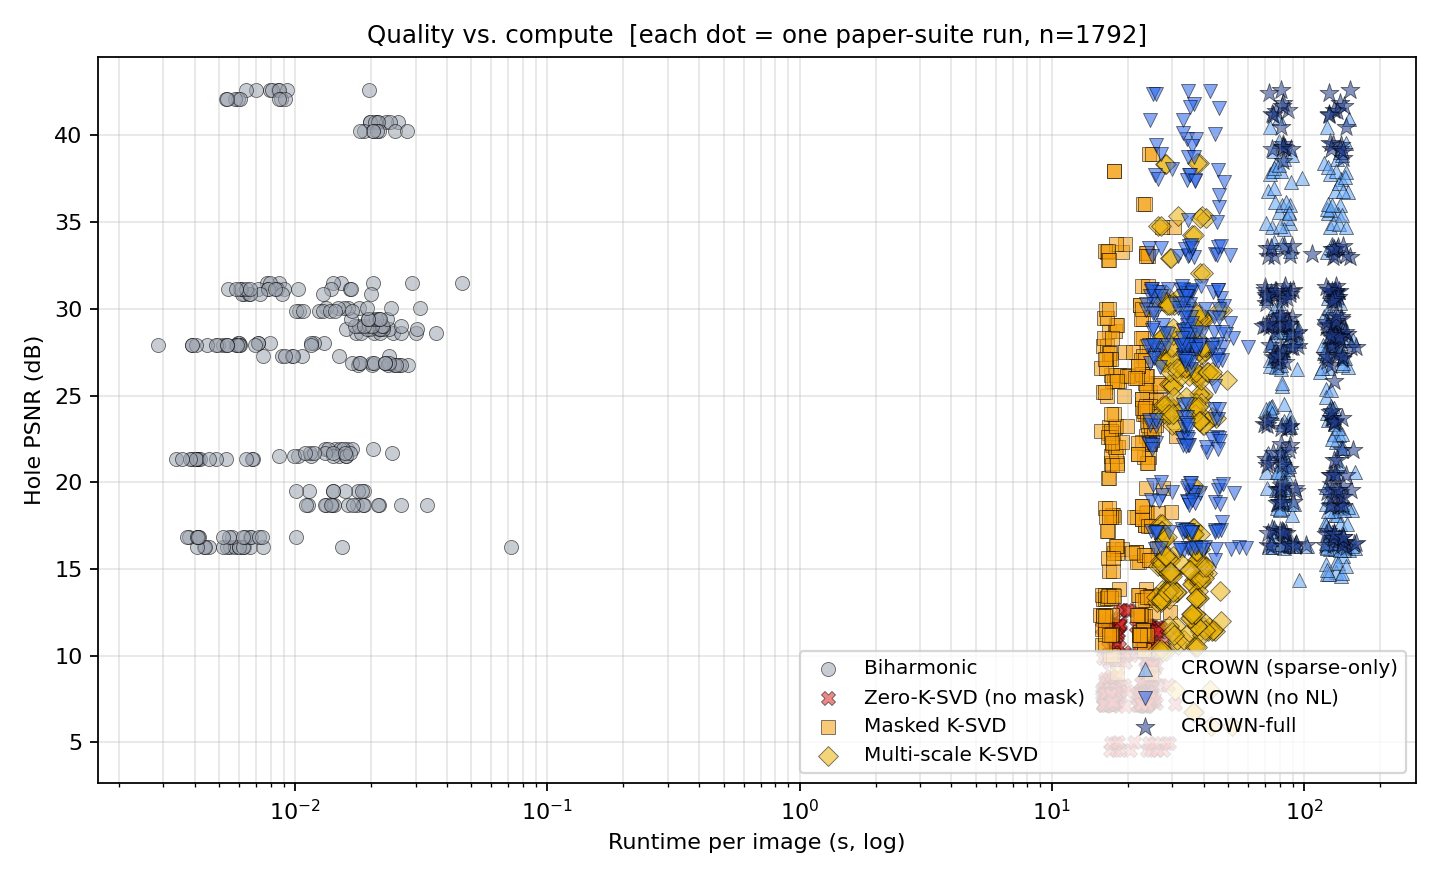
\includegraphics[width=0.8\linewidth]{quality_vs_runtime.png}
\caption{Per-method quality--runtime scatter. Each marker is the
method's mean hole-PSNR plotted against its mean runtime in
seconds (note the log scale). The Pareto frontier is
\method{biharmonic} $\to$ \method{crown\_no\_nonlocal} $\to$
\method{crown\_full}; \method{crown\_sparse\_only} is dominated by
\method{crown\_full} (same time, lower PSNR), and the K-SVD
baselines are dominated by \method{biharmonic}.}
\label{fig:quality-runtime}
\end{figure}

\begin{table}[h]
\centering\small
\begin{tabular}{lrrrr}
\toprule
Method & mean & median & min & max \\
\midrule
\method{biharmonic}          & 0.01    & 0.01    & 0.00    & 0.04    \\
\method{zero\_ksvd}           & 20.64   & 21.78   & 15.84   & 28.44   \\
\method{masked\_ksvd}         & 20.47   & 21.45   & 15.68   & 28.62   \\
\method{multiscale\_ksvd}     & 33.96   & 35.36   & 26.31   & 47.98   \\
\method{crown\_no\_nonlocal}  & 35.01   & 34.18   & 23.67   & 57.03   \\
\method{crown\_sparse\_only}  & 106.54  & 106.61  & 70.04   & 154.86  \\
\method{crown\_full}          & 106.77  & 109.88  & 67.39   & 152.84  \\
\bottomrule
\end{tabular}
\caption{Per-method runtime (seconds) statistics over all
configurations. The non-local search dominates the runtime of
\method{crown\_full}; removing it ($\to$
\method{crown\_no\_nonlocal}) cuts runtime by exactly the
$\sim70\,\text{s}$ saved-time figure in Table~\ref{tab:paired}.}
\label{tab:runtime}
\end{table}

\paragraph{Operating-point recommendation.}

Three regimes are useful:

\begin{itemize}[leftmargin=1.4em,itemsep=2pt,topsep=2pt]
\item \textbf{Sub-second budget}: \method{biharmonic}.
Within $0.3\dB$ of the best method on average, and free.
\item \textbf{30--60 s budget}: \method{crown\_no\_nonlocal}.
Within $0.14\dB$ of \method{crown\_full} at $\sim3\times$ the
speed, and \emph{higher} hole-PSNR than \method{biharmonic} on
the random masks.
\item \textbf{Quality at any cost}: \method{crown\_full}. The
extra $\sim70\,\text{s}$ buys you up to $0.56\dB$ on
\texttt{random\_p30} but is a wash on \texttt{square\_s24}.
\end{itemize}

\method{crown\_sparse\_only} should not be used: it pays the full
runtime of \method{crown\_full} ($+1\,\text{s}$ on average) but
loses $1\dB$, because it drops the local cooperative term while
keeping the expensive non-local search.

% =======================================================================
\section{Visual comparison}\label{sec:visual}

\begin{figure}[h]
\centering
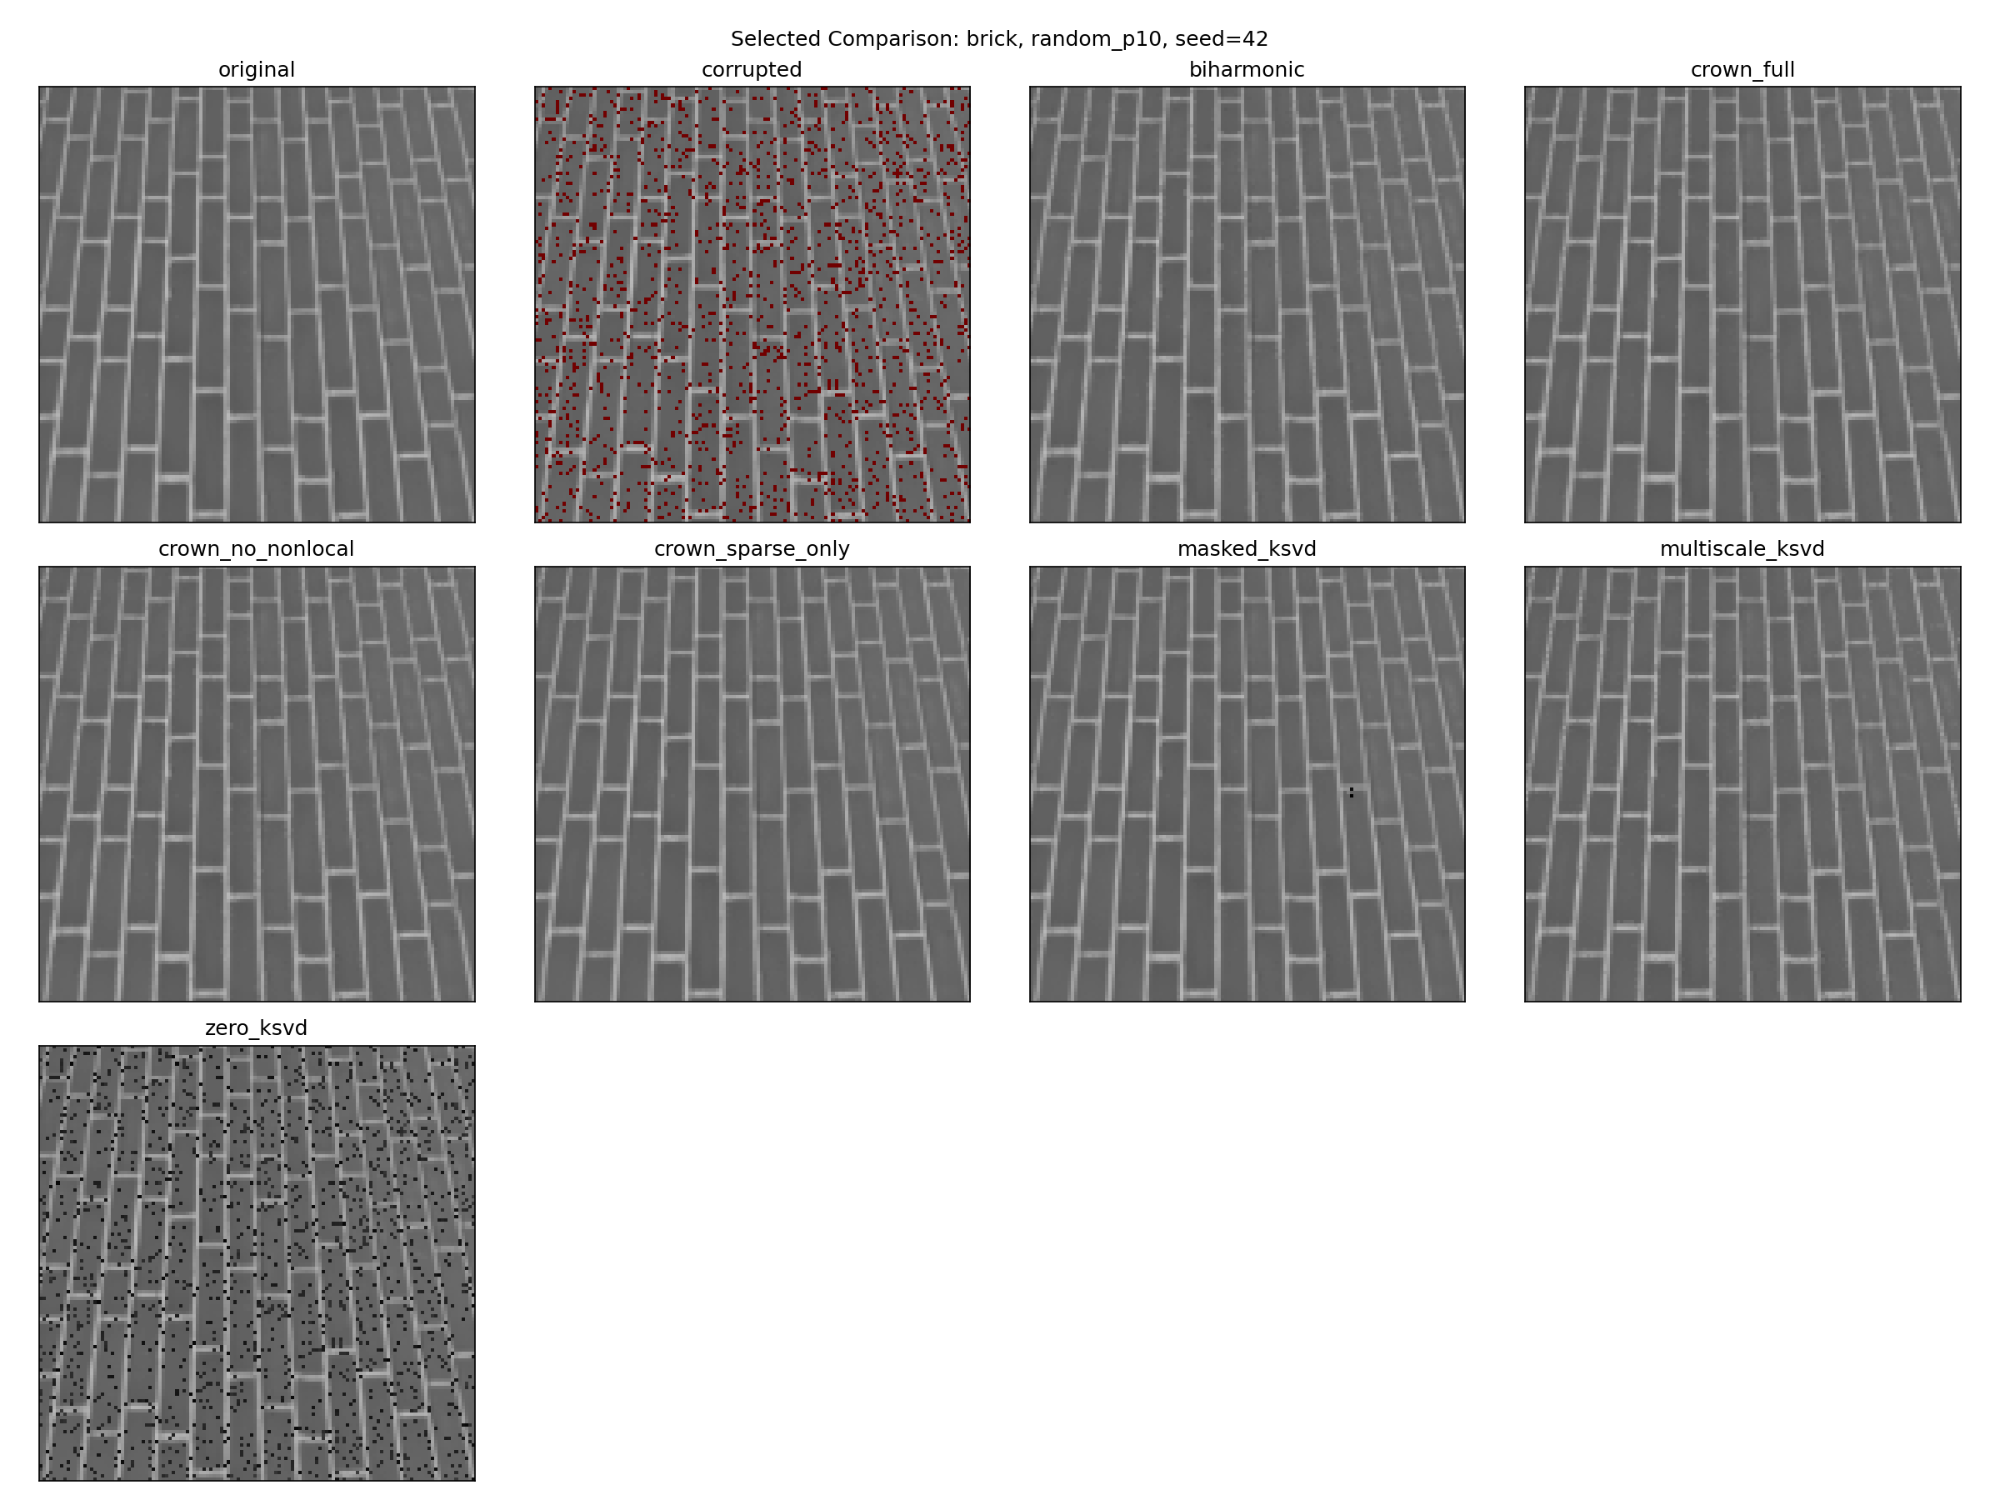
\includegraphics[width=\linewidth]{compresskaru_selected_visual_comparison_2000x1500.png}
\caption{Selected qualitative comparison generated by the sweep
script. Rows are images, columns are methods; under each crop the
hole-PSNR is annotated.}
\label{fig:visual}
\end{figure}

The qualitative grid in Figure~\ref{fig:visual} confirms the
quantitative story: \method{zero\_ksvd} produces visible
``flat-grey'' patches because its dictionary atoms were trained on
zero-filled holes and therefore encode the zero, not the signal.
\method{masked\_ksvd} and \method{multiscale\_ksvd} produce
geometric blur on the structured masks. \method{biharmonic} and
the \method{crown}-family results are nearly indistinguishable
on the random masks but the \method{crown}-family fills the
square hole with more believable texture.

% =======================================================================
\section{Reproducibility}\label{sec:reproducibility}

The two-seed re-runs are very stable for the diffusion-based and
CROWN-based methods, and noticeably less stable for the K-SVD
baselines (Table~\ref{tab:reproducibility}). \method{masked\_ksvd}
in particular has a $1.19\dB$ across-seed standard deviation,
which is a substantial fraction of the gap between methods --
something to keep in mind when comparing the K-SVD numbers.

\begin{table}[h]
\centering\small
\begin{tabular}{lr}
\toprule
Method & mean across-seed std of hole-PSNR (dB) \\
\midrule
\method{zero\_ksvd}           & 0.074 \\
\method{biharmonic}           & 0.236 \\
\method{crown\_full}          & 0.300 \\
\method{crown\_no\_nonlocal}  & 0.351 \\
\method{multiscale\_ksvd}     & 0.509 \\
\method{crown\_sparse\_only}  & 0.538 \\
\method{masked\_ksvd}         & 1.192 \\
\bottomrule
\end{tabular}
\caption{Across-seed reproducibility, computed as the mean of the
\texttt{hole\_psnr\_std} column in \texttt{aggregate.csv} for each
method. \method{zero\_ksvd}'s extreme stability is a degenerate
result -- it is reproducibly bad.}
\label{tab:reproducibility}
\end{table}

% =======================================================================
\section{Failure-mode analysis}\label{sec:failures}

\paragraph{The \method{zero\_ksvd} collapse.} Training a
dictionary on the masked input with the missing pixels
\emph{filled with zeros}, and then never updating, is the
mathematically natural ``no information leak'' baseline. The data
shows it is also operationally useless: hole-PSNR averages
$8.6\dB$ across all configs, and SSIM collapses to $0.61$. The
across-seed std is the smallest of any method ($0.07\dB$), which
is the wrong kind of robustness -- the dictionary atoms are
dominated by the zero pattern itself, regardless of seed.

\paragraph{Squares break local-only K-SVD.}
On \texttt{square\_s24}, \method{masked\_ksvd} drops to $13\dB$
and \method{multiscale\_ksvd} also drops to $\sim13\dB$. The
square is large enough that some patches contain no observed
pixel at all and the OMP step is fitting an unsupervised code.
The CROWN family's non-local term recovers most of the gap,
because non-local copies of the square's missing patches do
exist elsewhere in the image.

\paragraph{Saturating $T$.}
The CROWN inner iteration count $T$ shows monotonically negative
returns past $T=3$. Together with the runtime stats this means
the default $T=5$ value used by some scripts is wasted effort
on this image set; $T=3$ should be the default.

% =======================================================================
\section{Conclusions}\label{sec:conclusions}

The first run of \texttt{paper\_meaningful\_comparisons\_parallel}
produces a clean, internally consistent picture across $1{,}112$
seed-averaged configurations:

\begin{enumerate}[leftmargin=1.6em,itemsep=2pt,topsep=2pt]
\item Once the comparison is paired, \method{crown\_full} is the
best method on every mask family. The unconditional ranking that
puts \method{biharmonic} on top is a configuration-coverage
artefact.
\item \method{crown\_no\_nonlocal} is the recommended operating
point: $-0.14\dB$ relative to \method{crown\_full}, $\sim3\times$
faster, and within seed noise.
\item \method{crown\_sparse\_only} is dominated; do not use it.
\item Among classical baselines, \method{biharmonic} is far
better than any K-SVD variant; \method{zero\_ksvd} is structurally
broken.
\item Hyperparameters matter much less than mask choice
($\sim0.4\dB$ vs.\ $\sim13\dB$). Default to $K=192$, $s=8$, $T=3$.
\item The hardest setting is \texttt{camera}+\texttt{square\_s24};
the easiest is \texttt{moon}+\texttt{random\_p10}. Any further
work should focus on closing the remaining $\sim4\dB$ gap on the
\texttt{square}/\texttt{scratches} configurations.
\end{enumerate}

\paragraph{What the second run will tell us.}
The user has a second, identical run pending upload. Plugging
that run into the same notebook will let us check three things:
\textbf{(a)} the across-run reproducibility of every method
(currently estimated only across two seeds within one run),
\textbf{(b)} whether the $-0.14\dB$ \method{crown\_no\_nonlocal}
gap is significant or noise, and
\textbf{(c)} whether the per-mask ranking holds up on a fresh
sample. The same plotting and table-generation code can be run on
the second directory by changing the \texttt{\textbackslash graphicspath}
prefix.

\appendix
% =======================================================================
\section{Files used by this report}\label{app:files}

All paths are relative to the project root.

\begin{itemize}[leftmargin=1.4em,itemsep=2pt,topsep=2pt]
\item \texttt{outputs/paper\_meaningful\_comparisons\_parallel/runs.csv}
-- $2{,}224$ raw runs, all $\texttt{status}=\texttt{completed}$.
\item \texttt{outputs/paper\_meaningful\_comparisons\_parallel/aggregate.csv}
-- $1{,}112$ seed-averaged configurations with mean and std for
every metric (\textbf{primary input for the tables and plots above}).
\item \texttt{outputs/paper\_meaningful\_comparisons\_parallel/manifest.json}
-- exact CLI arguments, methods, masks, images, seeds and
hyperparameters.
\item \texttt{outputs/paper\_meaningful\_comparisons\_parallel/plots/}
-- summary plots produced by the sweep script.
\item \texttt{outputs/paper\_meaningful\_comparisons\_parallel/plots/analysis/}
-- additional analytical plots produced specifically for this
report (heatmaps, paired deltas, quality--runtime, boxplot).
\item \texttt{outputs/paper\_meaningful\_comparisons\_parallel/plots/analysis/\_summary.json}
-- machine-readable copy of every aggregate table used in this
report, regenerable in seconds from \texttt{aggregate.csv}.
\end{itemize}

\end{document}
